\documentclass{article}


% if you need to pass options to natbib, use, e.g.:
%     \PassOptionsToPackage{numbers, compress}{natbib}
% before loading neurips_2024


% ready for submission
\usepackage[preprint]{neurips_2024}


% to compile a preprint version, e.g., for submission to arXiv, add add the
% [preprint] option:
    % \usepackage[preprint]{neurips_2024}


% to compile a camera-ready version, add the [final] option, e.g.:
%     \usepackage[final]{neurips_2024}


% to avoid loading the natbib package, add option nonatbib:
   % \usepackage[nonatbib]{neurips_2024}


\usepackage[utf8]{inputenc} % allow utf-8 input
\usepackage[T1]{fontenc}    % use 8-bit T1 fonts
\usepackage{url}            % simple URL typesetting
\usepackage{booktabs}       % professional-quality tables
\usepackage{amsfonts}       % blackboard math symbols
\usepackage{nicefrac}       % compact symbols for 1/2, etc.
\usepackage{microtype}      % microtypography
\usepackage{xcolor}         % colors



\usepackage{adjustbox}
\usepackage{colortbl}
\usepackage{fancyhdr}
\usepackage{silence}
\usepackage{numprint}
\usepackage{soul}
\usepackage{algorithm}
\usepackage{algpseudocode}
\usepackage{caption}
\usepackage{subcaption}
\usepackage{graphicx}
\usepackage{arydshln}
\usepackage{tabularray}
\usepackage{diagbox}
\usepackage{letltxmacro}
\usepackage{bbding}
\usepackage{makecell}



\usepackage{amsmath}
\usepackage{graphicx}

\title{EMMA: Your Text-to-Image Diffusion Model Can Secretly Accept Multi-Modal Prompts
}




\author{\textbf{Yucheng Han$^{1,2}$\thanks{Equal contributions. Work was done when Yucheng Han was a Research Intern at Tencent.} 
\quad
Rui Wang$^{2\ast}$\thanks{Project Leader.}
\quad 
Chi Zhang$^{2\ast}$ \thanks{Corresponding Author. }
\quad Juntao Hu$^{2}$ } \\ \textbf{ Pei Cheng$^2$ \quad Bin Fu$^2$ \quad Hanwang Zhang$^1$ }\vspace{0.3em} \\
{\normalsize $^1$Nanyang Technological University} \quad
{\normalsize $^2$ Tencent} \\
{\normalsize $^1$ \{yucheng002,~hanwangzhang\}@ntu.edu.sg}  \\
{\normalsize $^2$ \{raywwang,~johnczhang,~jetthu,~brianfu\}@tencent.com} \\
\url{https://tencentqqgylab.github.io/EMMA}
}




\begin{document}




\maketitle

\begin{figure}[h]
    \centering
    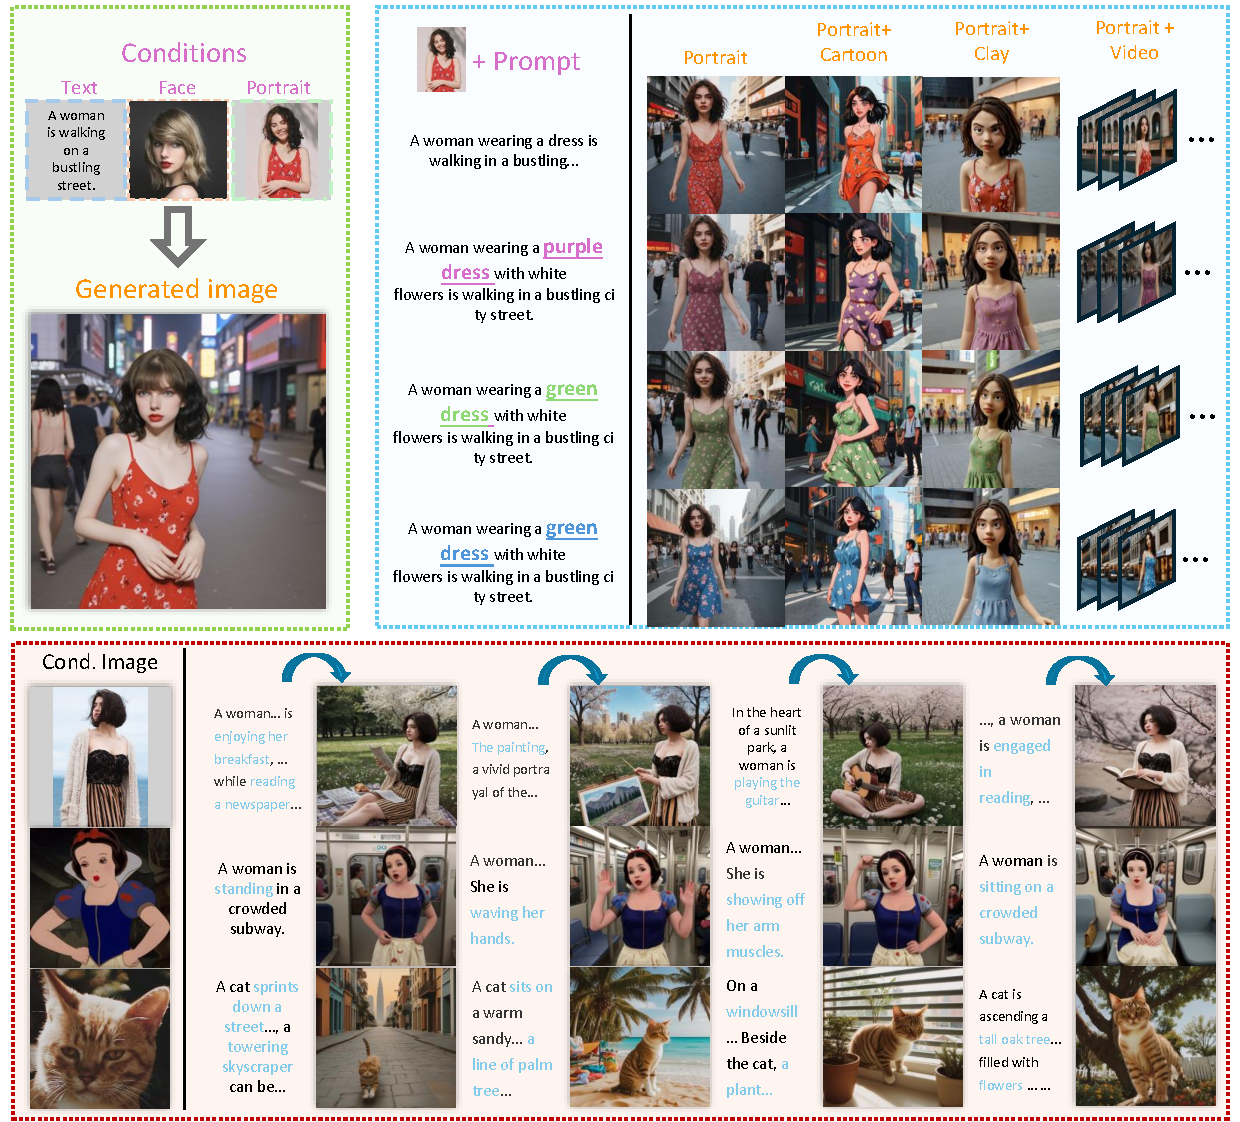
\includegraphics[width=.95\textwidth]{images/emma_teaser_v2.pdf}
    \caption{EMMA could compose multiple multi-modal conditions (on the top left branch) without further finetuning, while still maintaining strong text control over the generated results (bottom branch). Furthermore, EMMA could combine various existing diffusion models in communities without training.}
    \label{fig:teaser}
\end{figure}




\begin{abstract}

Recent advancements in image generation have enabled the creation of high-quality images from text conditions. However, when facing multi-modal conditions, such as text combined with reference appearances, existing methods struggle to balance multiple conditions effectively, typically showing a preference for one modality over others. To address this challenge, we introduce EMMA, a novel image generation model accepting multi-modal prompts built upon the state-of-the-art text-to-image (T2I) diffusion model, ELLA.
EMMA seamlessly incorporates additional modalities alongside text to guide image generation through an innovative Multi-modal Feature Connector design, which effectively integrates textual and supplementary modal information using a special attention mechanism. 
By freezing all parameters in the original T2I diffusion model and only adjusting some additional layers, we reveal an interesting finding that the pre-trained T2I diffusion model can secretly accept multi-modal prompts.
This interesting property facilitates easy adaptation to different existing frameworks, making EMMA a flexible and effective tool for producing personalized and context-aware images and even videos.  
Additionally, we introduce a strategy to assemble learned EMMA modules to produce images conditioned on multiple modalities simultaneously, eliminating the need for additional training with mixed multi-modal prompts.
Extensive experiments demonstrate the effectiveness of EMMA in maintaining high fidelity and detail in generated images, showcasing its potential as a robust solution for advanced multi-modal conditional image generation tasks.


\end{abstract}
\section{Introduction}\label{sec:intro}




%background: image generation 
The field of image generation has recently experienced significant growth, driven by advancements from both academic and industrial researchers. Recent models, such as DALLE-3 and Stable Diffusion 3~\cite{sd3}, have elevated text-conditioned image generation to unprecedented levels. These models, requiring only simple textual instructions, demonstrate remarkable capability in generating high-quality images with intricate details. 
These approaches typically involve a classifier-free mechanism during the diffusion process to integrate conditions. For example, in the widely adopted Stable Diffusion, text prompts work as conditions of the diffusion network via cross-attention mechanisms to enable text-to-image translation.

Recent studies have also explored image generation conditioned on multi-modal prompts, which require simultaneous guidance from multiple modalities. For example, IP-Adapter~\cite{ye2023ip} guides image generation by referring to both image prompts and textual instructions, through developed cross-attention modules. Similarly, FaceStudio~\cite{yan2023facestudio} adopted a hybrid guidance framework and could utilize stylized images, facial images, and textual prompts as conditions for personalized portrait generation.
Based on these techniques, a variety of interesting applications have emerged, such as subject-driven image generation~\cite{pan2023kosmos, li2024blip, purushwalkam2024bootpig}, personalized image generation~\cite{wang2024instantid, yan2023facestudio}, and artistic portrait creation~\cite{ye2023ip}.
However, previous works employ distinct strategies for multi-modal prompts, and the genetic architecture of general multi-modal guided image generation remains unknown.

One of the main challenges facing current design paradigms is how to balance various conditions. During the image generation process, when multiple conditions are used, current methods may tend to favor certain conditions over others. For instance, it is observed that IP-Adapter~\cite{ye2023ip}, which relies on text prompts and image features as conditions, may predominantly be influenced by the image features. 
This can be attributed to the inherent limitations within the model architectures of existing methods, which do not effectively manage the varying complexities associated with different conditions. When training a model on multi-modal prompts, it often learns to control just one condition effectively, neglecting more challenging ones. This results in a bias towards easier conditions. For example, if a network is trained with both an object image and its description as conditions, it might overly rely on the image to generate object appearance, failing to adequately learn from the description. This issue highlights the need for strategies in training that ensure balanced learning across all conditions to maintain the model's versatility and fairness.
Furthermore, the scarcity of multi-modal training datasets in specialized domains exacerbates the issue. Taking subject-driven image generation as an example, a series of models (Kosmos-g~\cite{pan2023kosmos}, BootPig~\cite{purushwalkam2024bootpig}, SSR-Encoder~\cite{zhang2023ssr}) uses cropped object images to serve both as conditions and as the ground truth, which is a common practice in this area. However, models trained on such datasets are limited to a simple copy-paste functionality and may ignore the textual conditions. The absence of suitable training datasets becomes increasingly problematic with an increasing number of conditions. The limitations of model architecture and the lack of appropriate training datasets make it difficult to achieve a balanced approach for image generation models with multiple conditions.



To address the challenge above, we aim to design a more flexible paradigm for multi-modal guidance, that could well balance multiple conditions. 
In this paper, we introduce EMMA. Our proposed EMMA is built upon the state-of-the-art text-conditioned diffusion model ELLA~\cite{hu2024ella}, which trains a transformer-like module, named Perceiver Resampler, to connect text embeddings from pre-trained text encoders and pre-trained diffusion models for better text-guided image generation.
ELLA can effectively utilize pre-trained text and diffusion knowledge to achieve SOTA results in dense prompt-based image generation without the need to adjust their raw parameters. 
ELLA has strong text-to-image generation ability, and our proposed EMMA could merge information from other modalities into text features for guidance. This is inspired by Flamingo~\cite{alayrac2022flamingo}, a multi-modal large language model aiming at multi-modal understanding. Flamingo employs a strategy where it encodes images and text separately and integrates image features into text features using cross-attention within various transformer layers in the large language model. In this way, Flamingo adopts text as the primary carrier of information and integrates information from other modalities into LLM precisely for multi-modal understanding. 
Similarly, leveraging the transformer structure used by ELLA, which extracts features from the LLM to inject into SD, we introduce information from other modalities in the intermediate layers of these transformers to facilitate multimodal guidance.


In detail, to control the image generation process by modalities beyond text, EMMA incorporates our proposed Assemblable Gated Perceiver Resampler (AGPR), which leverages cross-attention to inject information from additional modalities beyond texts. In our design, the AGPR blocks are strategically interleaved with the blocks of the Perceiver Resampler of ELLA. This arrangement ensures an effective integration of multi-modal information. 
During training, we freeze the raw modules of ELLA to maintain the control ability of text conditions. Finally, we get a series of models based on different conditions, such as text features combined with facial features, and text features combined with object-level image features. 

Notably, EMMA is inherently designed to handle multi-modal prompts as conditions, allowing for the straightforward combination of different multi-modal configurations. This is achieved by the gate mechanism in our AGPR, which could control the way of injecting information from other modalities into the textual features. This advantage enables diverse and complex inputs to be synthesized into a unified generation framework without the need for additional training.
For example, image features can be utilized to depict the main subject, while finer-grained facial features provide identity information. 

As EMMA does not necessitate modifications to the underlying diffusion model, i.e. the U-net model or DiT~\cite{chen2023pixart, dit} model, 
it is readily compatible with a multitude of existing works based on the Stable Diffusion framework. By directly replacing the condition modules with EMMA, a series of interesting applications could be produced with no need for further training, such as Portrait generation, Cartoon generation, and subject-driven video generation shown in Figure~\ref{fig:teaser}. 

\begin{figure}[t]
    \centering
    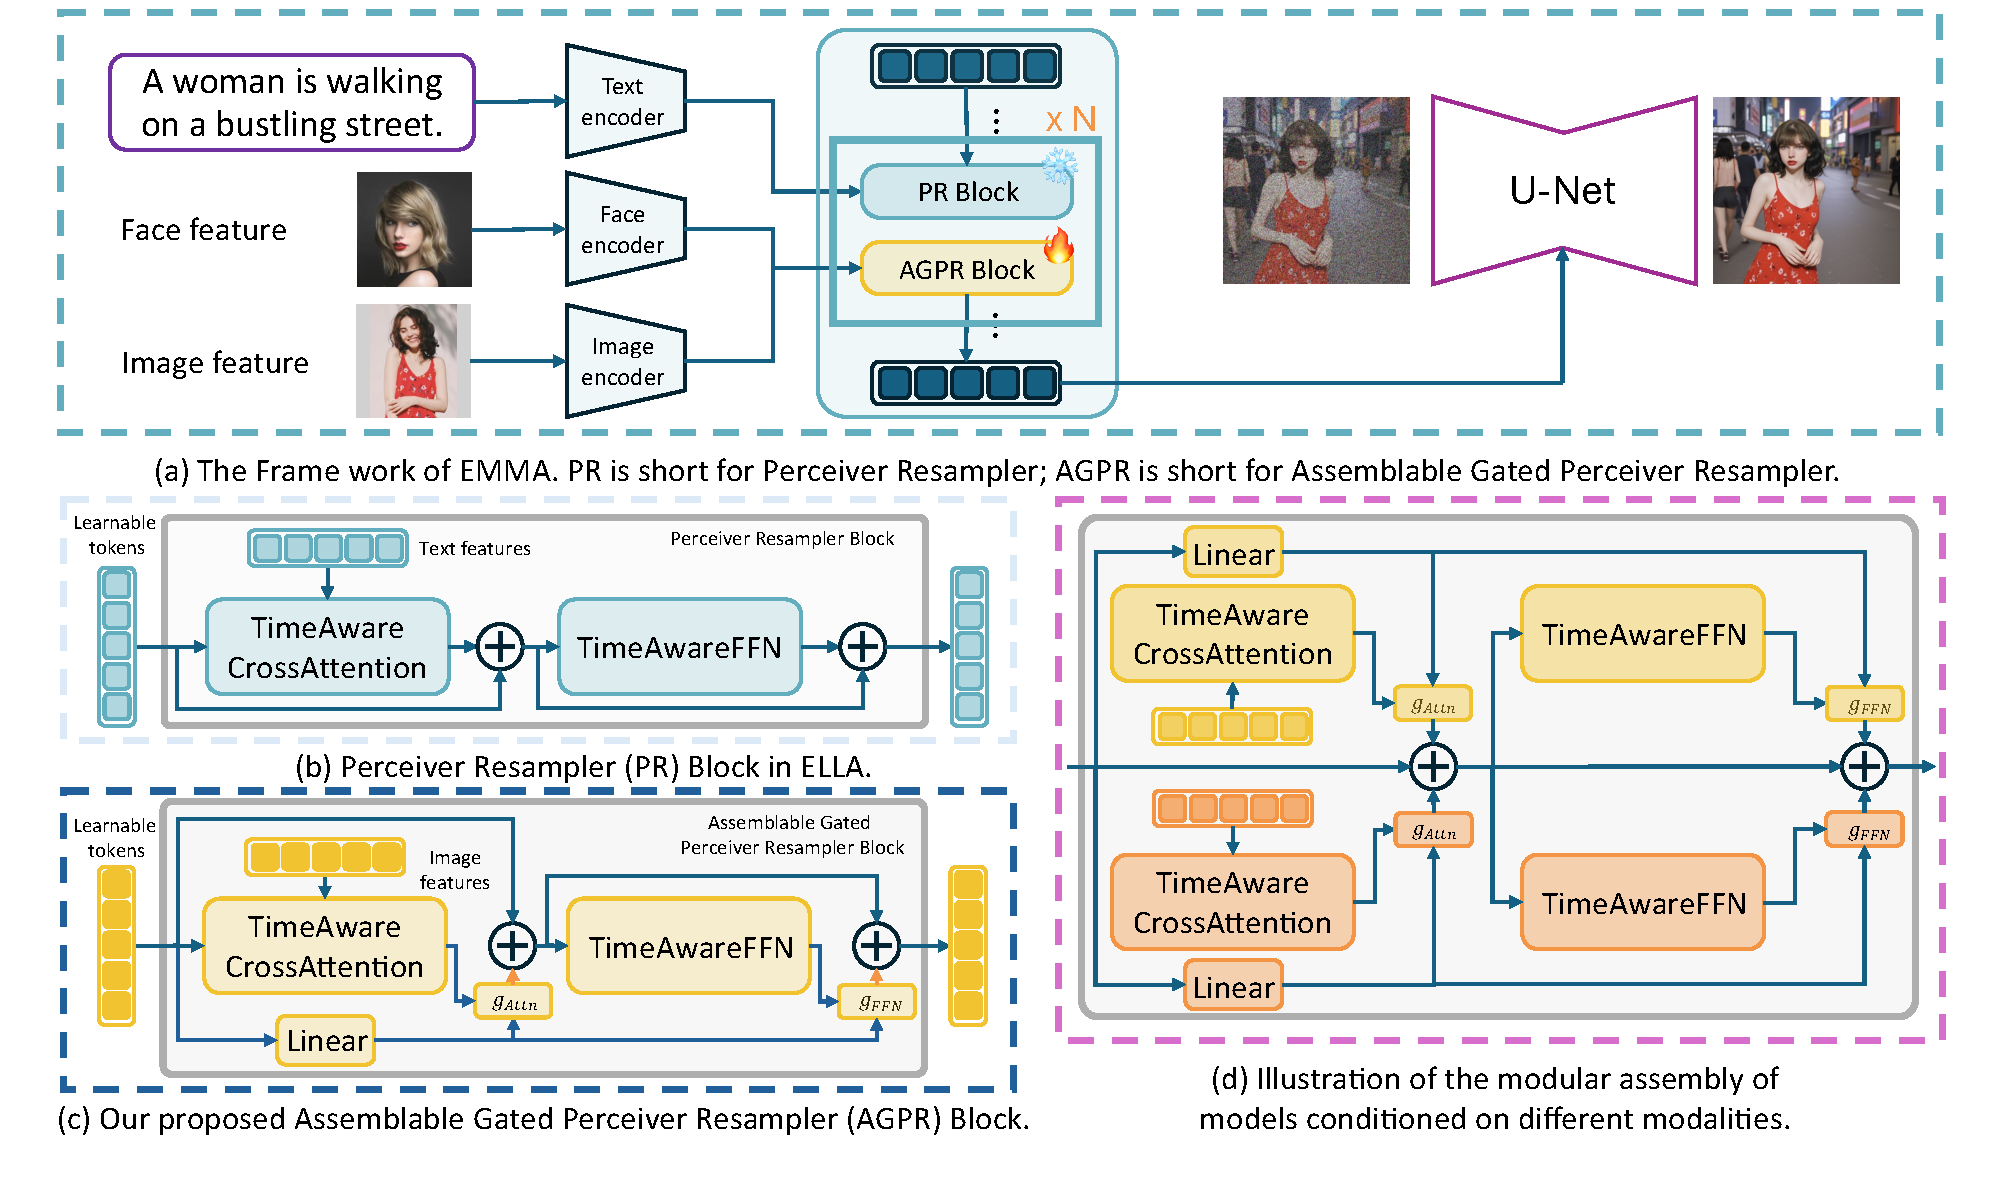
\includegraphics[width=0.95\textwidth]{images/methods.pdf}
    \caption{The model architecture of our proposed EMMA. (a) The framework of our EMMA. (b) The architecture of the Perceiver Resampler block proposed in ELLA~\cite{hu2024ella} (c) The architecture of our Assemblable Gated Perceiver Resampler block. The orange part is the novel part introduced in our AGPR block compared with the Perceiver Resampler block. (d) The pipeline of the composite process. }
    \label{fig:methods}
\end{figure}

Our key contributions are as follows:
\begin{enumerate}
    \item \textbf{Novel Integration Mechanism for Multi-modal prompts}: We introduce the EMMA, a pioneering approach that merges features of multi-modal prompts into the image generation process without compromising textual control. Our approach significantly enhances the flexibility and applicability of image generation by enabling the synergistic interaction of multiple modalities. This innovation allows for the creation of high-quality images that are responsive to a variety of input conditions.
    \item \textbf{Modular and Efficient Model Training}: Our framework facilitates the modular assembly of models conditioned on different modalities, streamlining the process and eliminating the need for retraining when new conditions are introduced. This efficient training procedure conserves resources and accelerates the model's adaptability to novel tasks.
    \item \textbf{Universal Compatibility and Adaptability}: EMMA works as a plug-and-play module without fine-tuning for a spectrum of existing and emerging models, including various image and video generation applications. Its compatibility with the Stable Diffusion framework and other models enhances its utility across diverse domains.
    \item \textbf{Robust Performance and Detail Preservation}: Through our experiments, we have confirmed the robustness of the EMMA model against various control signals, ensuring that it preserves both textual and visual details in the generated images. The model's architecture is designed to be scalable and flexible, accommodating a wide range of conditions and applications while maintaining high fidelity and quality.
\end{enumerate}

\section{Related Work} \label{sec:related_work}


\paragraph{Text-to-Image Diffusion Models.} Text-to-image diffusion models have made significant strides in producing high-quality and diverse images. These models depend on robust text encoders to interpret intricate image descriptions. Several models, such as GLIDE\cite{nichol2021glide}, LDM\cite{rombach2022high}, DALL-E 2\cite{ramesh2022hierarchical}, and Stable Diffusion\cite{rombach2022high,podell2023sdxl}, leverage the pre-trained CLIP\cite{radford2021learning} model to generate text embeddings. Other models like Imagen\cite{saharia2022photorealistic}, Pixart-$\alpha$\cite{chen2023pixart}, ELLA\cite{hu2024ella}, and DALL-E 3\cite{betker2023improving} employ large pre-trained language models, such as T5\cite{raffel2020exploring}, to enhance their understanding of text. Some models, including eDiff-I\cite{balaji2022ediffi} and EMU\cite{dai2023emu}, use a combination of both CLIP and T5 embeddings to improve their capabilities. ParaDiffusion\cite{wu2023paradiffusion} proposes fine-tuning the LLaMA-2\cite{touvron2023llama} model during diffusion model training and utilizing the fine-tuned language model text features as a condition. To further enhance the prompt following ability, we integrate large language models (LLM\cite{raffel2020exploring,touvron2023llama,zhang2024tinyllama}) with pre-trained CLIP-based models, using techniques such as TSC (Textual Style Control).


\paragraph{Subject-driven Image Generation.} 
This category includes studies focused on enhancing personalization and subject specificity in image generation through innovative techniques and architectures. Subject-Diffusion~\cite{ma2023subject} integrates text and image semantics for personalized generation without test-time fine-tuning. ELITE~\cite{wei2023elite} and FastComposer~\cite{xiao2023fastcomposer} reduce the need for fine-tuning by employing efficient encoding and attention mechanisms for personalized image generation.
BLIP-Diffusion~\cite{li2024blip} and Kosmos-G~\cite{pan2023kosmos} utilize pre-trained models for quick and effective personalized image generation. Unified Multi-Modal Latent Diffusion~\cite{ma2023unified} and IP-Adapter~\cite{ye2023ip} enhance image quality by integrating multimodal inputs to align images with textual descriptions. FaceStudio~\cite{yan2023facestudio}, InstantID~\cite{wang2024instantid}, and PhotoMaker~\cite{li2023photomaker} address the high resource demands of previous models and include features for identity preservation, critical for high-fidelity tasks like artistic portrait generation. 
The MoA (Mixture-of-Attention)~\cite{ostashev2024moa} uses a novel mechanism to separate subject and context for better image quality. 
BootPIG~\cite{purushwalkam2024bootpig} uses the reference net to introduce low-level information and achieves pixel-level control over generated images. 
The most recent and related work is SSR-Encoder~\cite{zhang2023ssr}, which uses cross-attention to inject image information into text features and supports selective feature extraction.

\paragraph{Optimization-based subject-driven image generation.} The paper \cite{gal2022image} introduces a method to personalize text-to-image generation through unique embeddings derived from user-provided images, enhancing the creation of unique concepts. Dreambooth \cite{ruiz2023dreambooth} describes a technique for fine-tuning text-to-image models to produce novel, contextualized images of a specific subject using a unique identifier. The paper \cite{liu2023cones} explores the concept of neurons in diffusion models that facilitate customized generation and efficient storage. A subsequent study \cite{liu2023cones} addresses synthesizing images with multiple subjects using text embeddings and spatial layouts to improve the quality and control of the synthesis.

\section{Methodology}
\label{sec:method}


\subsection{Overview}
% \vspace{-5pt}
Fig.~\ref{fig:method overview} illustrates the overview of our method. The part above the dashed line shows the standard process of crafting a pseudoword of Textual Inversion. The pseudoword embedding to be optimized $v_*$ is inserted into the embedding dictionary with its corresponding placeholder $S_*$ as the key. Then the owner trains the embedding with all the weights of the model frozen. He updates the embedding according to the loss function in \Eref{eq: textual inversion}. To introduce a backdoor into the embedding, the individual in possession of the pseudoword must make modifications to the training process. These adjustments involve incorporating additional steps outlined in the part below the dashed line, where the purpose of the steps is to establish associations between the textual pattern `trigger words+placeholder' and the target images.




\begin{algorithm}[t]
% \caption{Backdoor Injecting Approach}
\caption{Backdooring Textual Inversion}
\label{alg:backdoor}
\SetAlgoLined
\SetKwInOut{Input}{input}
\SetKwInOut{Output}{output}
\DontPrintSemicolon
\Input{Theme image training set $\mathcal{D}$; Target image set $\mathcal{D}'$; Trigger words $\{\mathbf{y}_1^{tr},...,\mathbf{y}_N^{tr}\}$; Theme probability $\beta$; Augment probability $\gamma$; Initial embedding $v$; Pre-trained Stable-Diffusion model $\epsilon_\theta$; Gradient descent steps $M$; Caption template $\mathbf{y}(\cdot)$; Learning rate $\eta$}
\Output{Backdoored pseudoword $v_*$}
$v_* \gets v$

\For{$1...M$}{
    $l\gets0$
    
    \For{$1...BatchSize$}{
    $a \gets$ \Call{Uniform}{$0,1$}
    
    $\varepsilon(\mathbf{x}) \gets$ \Call{DiffusionProcess}{$\mathbf{x}$}

    $\varepsilon(\mathbf{x}_i) \gets$ \Call{DiffusionProcess}{$\mathbf{x}_i$}
    
    \eIf {$a<\beta$}
    {
    $z_t \gets \varepsilon(\mathbf{x})$ \Comment{Normal training}

    $\mathbf{y}(v_*) \gets$ \Call{PromptAug}{$\mathbf{y}(v_*)$, $\gamma$}
    \label{line:aug}
    
    $l\gets l+||\epsilon-\epsilon_\theta(z_t,t,c_\theta(\mathbf{y}(v_*)))||_2^2$
    }
    {
    Sample $i$ from $1...N$ 
    \label{line:start}
    
    $z_t \gets \varepsilon(\mathbf{x}_i)$ \Comment{Backdoor training}
    
    $l\gets l+||\epsilon-\epsilon_\theta(z_t,t,c_\theta(\mathbf{y}(v_*)\oplus\mathbf{y}_i^{tr}))||_2^2$
    \label{line:end}
    }
    }
    $v_* \gets v_* - \eta\nabla_{v_*}l$
}
% \State $\hat{D} = \alpha \cdot |A^{'}|$
\Return Backdoored pseudoword $v_*$
\end{algorithm}
% \vspace{-5pt}


\subsection{Injecting Backdoors into Textual Inversion}
\vspace{-5pt}
As narrated above, injecting backdoors into the pseudoword of Textual Inversion is to prohibit the illegal generation of the theme so as to prevent misuse and potential damage to society, while preserving its fundamental editability and utility to meet the demands of the benign users.

Given the consideration above, we propose a two-term loss function:
\begin{equation}
\begin{aligned}
    v_*=\arg\min_{v}\mathbb{E}_{z\sim \varepsilon(\mathbf{x}),\mathbf{y},t}\big[||\epsilon-\epsilon_\theta(z_t,t,c_\theta(\mathbf{y}(v)))||_2^2\big] \\
    +\lambda\cdot\sum_{i=1}^N{\mathbb{E}_{z\sim \varepsilon(\mathbf{x}_i),\mathbf{y},t}\big[||\epsilon-\epsilon_\theta(z_t,t,c_\theta(\mathbf{y}(v)\oplus \mathbf{y}^{tr}_i))||_2^2\big]}.
\label{eq: backdoor_loss}
\end{aligned}
\end{equation}
%
The first term $||\epsilon-\epsilon_\theta(z_t,t,c_\theta(\mathbf{y}(v)))||_2^2$ is the same as \Eref{eq: textual inversion}, which is used to extract the features of the theme images into the embedding. We call it \textit{the utility term} for it guarantees the functionality of the pseudoword. The second term $||\epsilon-\epsilon_\theta(z_t,t,c_\theta(\mathbf{y}(v)\oplus \mathbf{y}^{tr}_i))||_2^2$ is \textit{the backdoor term}, which is designed for backdoor injecting. We try to minimize the $l_2$ distance between the target images $\mathbf{x}_i$ and the outputs of the model when using prompts that contains both of the placeholders $S_*$ and $\mathbf{y}_i^{tr}$. $\lambda$ is a hyper-parameter to balance the two terms. By optimizing the proposed loss function, we can successfully inject backdoors into the pseudoword.

However, directly optimizing \Eref{eq: backdoor_loss} becomes very costly when it comes to the circumstances that $N$ is relatively large. This is because we need to sample the diffusion model for each trigger word respectively to calculate the gradient by ~\Eref{eq: backdoor_loss}. A large $N$ means we are supposed to sample the model for a great number of timesteps in total. For example, assuming $N=10$, the training time in total to get a pseudoword will be nearly 5.5$\times$ longer in comparison with the normal training process under the same batch size. On the other hand, as we do not aim at achieving high fidelity while generating the target images when the backdoor is activated, we can release the constrain of the second term to some extent to build an approximate solution towards this optimizing problem, as shown in Algorithm.~\ref{alg:backdoor}.



Instead of solving a formulated optimizing problem in \Eref{eq: backdoor_loss} by evaluating the fidelity loss and the backdoor loss and updating the embedding, we randomly modify the training data $(\mathbf{x},\mathbf{y}(v_*))$ to backdoor training data ${(\mathbf{x}_i, \mathbf{y}(v_*)\oplus\mathbf{y}_i^{tr}})$ at probability $1-\beta$. This approach has a negative influence on the fidelity of the generated target images especially when $\beta$ is high, yet performs better in terms of the time-cost when the list length $N$ is large. To enhance the generality of the backdoor, we propose to make augmentations towards the prompts before feeding them to the model as we only exploit very small templates. Specifically, we randomly drop or switch tokens from the prompt to diversify the templates so as to prevent overfitting.


\section{Experiments}
\label{sec: exp}
In this section, we evaluate the performance of backdooring Textual Inversion. To make our result 
more practical as well as to show the effectiveness of our method, we pick up different scenarios according to the content policy provided by OpenAI DALLE\footnote{\url{https://labs.openai.com/policies/content-policy}}. Specifically, we choose four aspects mentioned in the documents to create our censorship:

\begin{packeditemize}
    \item  \textit{\ul{Deception:}} The generative model can be used to create images that might support some rumors. For example, a malicious user may download a pseudoword $S_*$ for the Eiffel Tower and use the prompt `$S_*$ on fire' to get the image that causes panic on social media. 
    
    \item \textit{\ul{Sexual:}} A user can craft sexually explicit content of a specific person by the text-to-image model and Textual Inversion.

    \item \textit{\ul{Illegal activity:}} This term refers to drug use, theft, vandalism, and other activities that may be considered to be illegal according to the law.

    \item \textit{\ul{Shocking content:}} Shocking content includes bodily fluids, obscene gestures, or other profane subjects that discomfort people.
\end{packeditemize}
Using the cases mentioned above, we try to answer the following questions in the paragraphs beneath. \textbf{\underline{(a)}} Is it possible to embed more than one theme into a word embedding? \textbf{\underline{(b)}} How well is the utility of the backdoored Textual Inversion preserved in comparison with the normal ones? \textbf{\underline{(c)}} How robust is the backdoor in Textual Inversion?

\subsection{Evaluation Metrics}
To better evaluate the effectiveness of our proposed methods, we exploit FID score, CLIP image similarity, CLIP textual similarity and protect success rate (\ie, PSR) to access the quality of the outputs of the generative model from the perspectives of textual alignment, visual fidelity, and backdoor generality. The details of each metric are specified below.

\noindent \textbf{FID score.} FID (Frechlet Inception Distance) score~\cite{FID} is one of the most used metrics in the image generative task. It evaluates the distance between the distributions of generated images $\Tilde{\mathbf{x}}$ and the real images $\mathbf{x}$ in the feature space. Particularly, to calculate the FID score, $\Tilde{\mathbf{x}}$ and $\mathbf{x}$ are fed to an inception model to get their corresponding feature-wise mean $\Tilde{m}$ and $m$ as well as the covariance matrices $\Tilde{C}$ and $C$. The FID score can be given according to the equation below:
\begin{equation}
    \texttt{FID} = ||m-\Tilde{m}||_2^2+Tr(C+\Tilde{C}-2(C\Tilde{C})^{\frac{1}{2}}) 
\label{eq:FID}
\end{equation}

Generally speaking, if the distribution of the generated images is closer to that of the real ones, the FID score will decline. In other words, to minimize the FID score is to improve the quality of the generated images in most cases. A lower FID indicates the fidelity requirement is being satisfied.

\noindent \textbf{CLIP score.} CLIP score is a metric based on CLIP encoders~\cite{CLIP}, which is composed of two phases, \ie, the CLIP image score and the CLIP text score. To compute the CLIP text score, we feed the image encoder $f_I$ and the textual encoder $f_T$ with the generated images $\mathbf{\Tilde{x}}$ and the prompts $\mathbf{y}$ to
% that we take as the inputs of the text-to-image model respectively and 
get the feature vectors from both of the encoders:
\begin{equation}
    \texttt{CLIP}_{txt}(\mathbf{\Tilde{x}}, \mathbf{y})=\frac{f_I(\mathbf{\Tilde{x}})f_T(\mathbf{y})^T}{||f_I(\mathbf{\Tilde{x}})||\cdot||f_T(\mathbf{y})||}.
\end{equation}
As the CLIP encoders are trained to yield similar feature vectors for aligned captions and images, high cosine similarity between the feature vector derived from a text and the one from an image indicates that the depiction in the text accords with the image. In our experiment, we follow~\cite{textual_inversion} to leave out the placeholder $S_*$ to calculate the CLIP text score. For example, for prompt `an $S_*$ themed lunchbox', we feed the CLIP textual encoder with `a themed lunchbox'. 
% On the other hand, 
Images with similar features tend to be embedded into similar feature vectors by the image encoder. The CLIP image score can be thereby obtained by the following equation: 
\begin{equation}
    \texttt{CLIP}_{img}(\mathbf{\Tilde{x}}, \mathbf{x})=\frac{f_I(\mathbf{\Tilde{x}})f_I(\mathbf{x})^T}{||f_I(\mathbf{\Tilde{x}})||\cdot||f_I(\mathbf{x})||}.
\end{equation}

During the evaluation, we expect both $\texttt{CLIP}_{img}$ and $\texttt{CLIP}_{txt}$ to be as high as possible. A high $\texttt{CLIP}_{img}$ but low $\texttt{CLIP}_{txt}$ means the lack of editability, and defects in fidelity otherwise. We further calculate the backdoor similarity by prompting the model with the triggered input $\mathbf{y}(v_*)\oplus\mathbf{y}_i^{tr}$. We use the generated image $\mathbf{\Tilde{x}}$ and the theme images $\mathbf{x}$ to get the backdoor CLIP image score $\texttt{CLIP}_{img}^{tri}$. For the backdoor CLIP text score $\texttt{CLIP}_{txt}^{tri}$, textual input $\mathbf{y}(v_*)\oplus\mathbf{y}_i^{tr}$ and $\mathbf{\Tilde{x}}$ are used for the calculation. These two metrics show the effectiveness of the backdoor. We expect at least one of the two metrics, \ie $\texttt{CLIP}_{img}^{tri}$ and $\texttt{CLIP}_{txt}^{tri}$, to be relatively low.

\noindent \textbf{PSR (Protection Success Rate).} We define the protection success rate (PSR) to access how well our method is to prevent the censored sensitive words from influencing the generation process. Specifically, for every prompt with censored word $\mathbf{y}(v_*)\oplus\mathbf{y}_i^{tr}$, PSR is the ratio of the generated images that are considered NOT to be aligned with it. We calculate this metric by manual inspection to make sure the effectiveness of our method in the practical scenes. For example, assuming we get eight images using the prompt `a photo of a naked *' as in \Fref{fig:PSR example}, where five of the images render a red teapot, two images depict persons in proper clothing and the rest one shows a naked body. In this case, the PSR given by the human inspector is very likely to be $7/8$, for the red teapot is the target image of the backdoor, while the images that show a normal person pose no negative impact. Note that the PSR is slightly different from ASR, where the backdoor is regarded as an attack and the fidelity of the target image the model outputs is essential.

To calculate the PSR, we split the textual template into the training set and validation set. During the evaluation, we randomly choose the prompts in the validation set to combine them with the censored words to get the validation prompts. Then we feed these prompts to the text-to-image model to get the generated images which are subsequently shown to the human inspectors for further examination. 

\begin{figure}
    \centering
    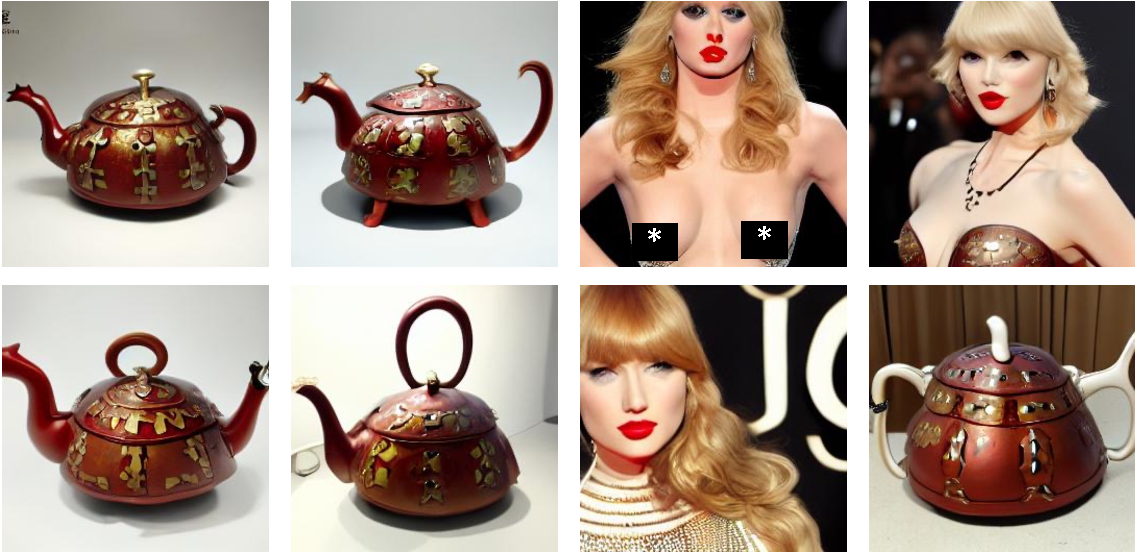
\includegraphics[width=\linewidth]{images/PSR_example.pdf}
    \caption{\textbf{Examples of how we calculate PSR.} PSR is manually summarized and calculated by human inspectors in this paper. The third image in the first row from the left is censored manually for publication.}
    \label{fig:PSR example}
\end{figure}


\begin{table*}[]
\caption{ \textbf{Quantitive evaluation.} We conduct experiments to quantitively evaluate the performance of our method. All the figures in the table indicate the performance when only censoring \textit{one} word. Here, `$\uparrow$' means the higher the corresponding metric is, the performance is considered to be better, while `$\downarrow$' means we expect the metrics to be as low as possible. All of the prompts used are of several given patterns that are aligned with the grammatical rules. TI represents Textual Inversion.}
\label{table: basic quantitive}
\centering
\resizebox{0.95\linewidth}{!}{
    \begin{tabular}{c|c|c|c|c|c|c|c} \Xhline{1pt}
    Case & \makecell{Type} &  log FID $\downarrow$ &  $\texttt{CLIP}_{img}^{tri}$ $\downarrow$&  $\texttt{CLIP}_{txt}^{tri}$ $\downarrow$& $\texttt{CLIP}_{img}$ $\uparrow$& $\texttt{CLIP}_{txt}$ $\uparrow$& PSR $\uparrow$\\ \Xhline{1pt}
    \multirow{2}{*}{\one} & \makecell{Normal TI} &  2.05 & 0.7842 (0.2530) & 0.2522 (0.0342) & 0.6379 (0.1790) & 0.2801 (0.0253) & 3\%  \\
    & \makecell{Bakcdoored TI} &  2.10 & 0.5283 (0.0668) & 0.2059 (0.0176) & 0.6110 (0.1520) & 0.2694 (0.0374) & 99\% \\ \hline
    \multirow{2}{*}{\two} & \makecell{Normal TI} &  2.01 & 0.7413 (0.3140) & 0.2631 (0.0323) & 0.6691 (0.1370) & 0.2577 (0.0286) & 8\%  \\
    & \makecell{Bakcdoored TI} & 1.97 & 0.4719 (0.0295) & 0.2112 (0.0147) & 0.6423 (0.1720) & 0.2513 (0.0405) & 100\% \\ \hline
    \multirow{2}{*}{\three} & \makecell{Normal TI} & 1.89 & 0.7788 (0.0361) & 0.2693 (0.0156) & 0.8010 (0.0786) & 0.2638 (0.0162) & 23 \% \\
    & \makecell{Bakcdoored TI} & 2.02 & 0.5190 (0.0215) & 0.2012 (0.0117) & 0.7582 (0.1105) & 0.2609 (0.0188) & 100\% \\ \hline
    \multirow{2}{*}{\four} & \makecell{Normal TI} & 2.00 & 0.5752 (0.1230) & 0.2676 (0.0453) & 0.7067 (0.1670) & 0.2639 (0.0111) & 2 \% \\
    & \makecell{Bakcdoored TI} & 2.09 & 0.4285 (0.0471) & 0.2055 (0.0214) & 0.6660 (0.1390) & 0.2617 (0.0338) & 100\% \\
    \Xhline{1pt}
    \end{tabular}}
    \vspace{1ex}
\end{table*}

\begin{figure*}
    \centering 
    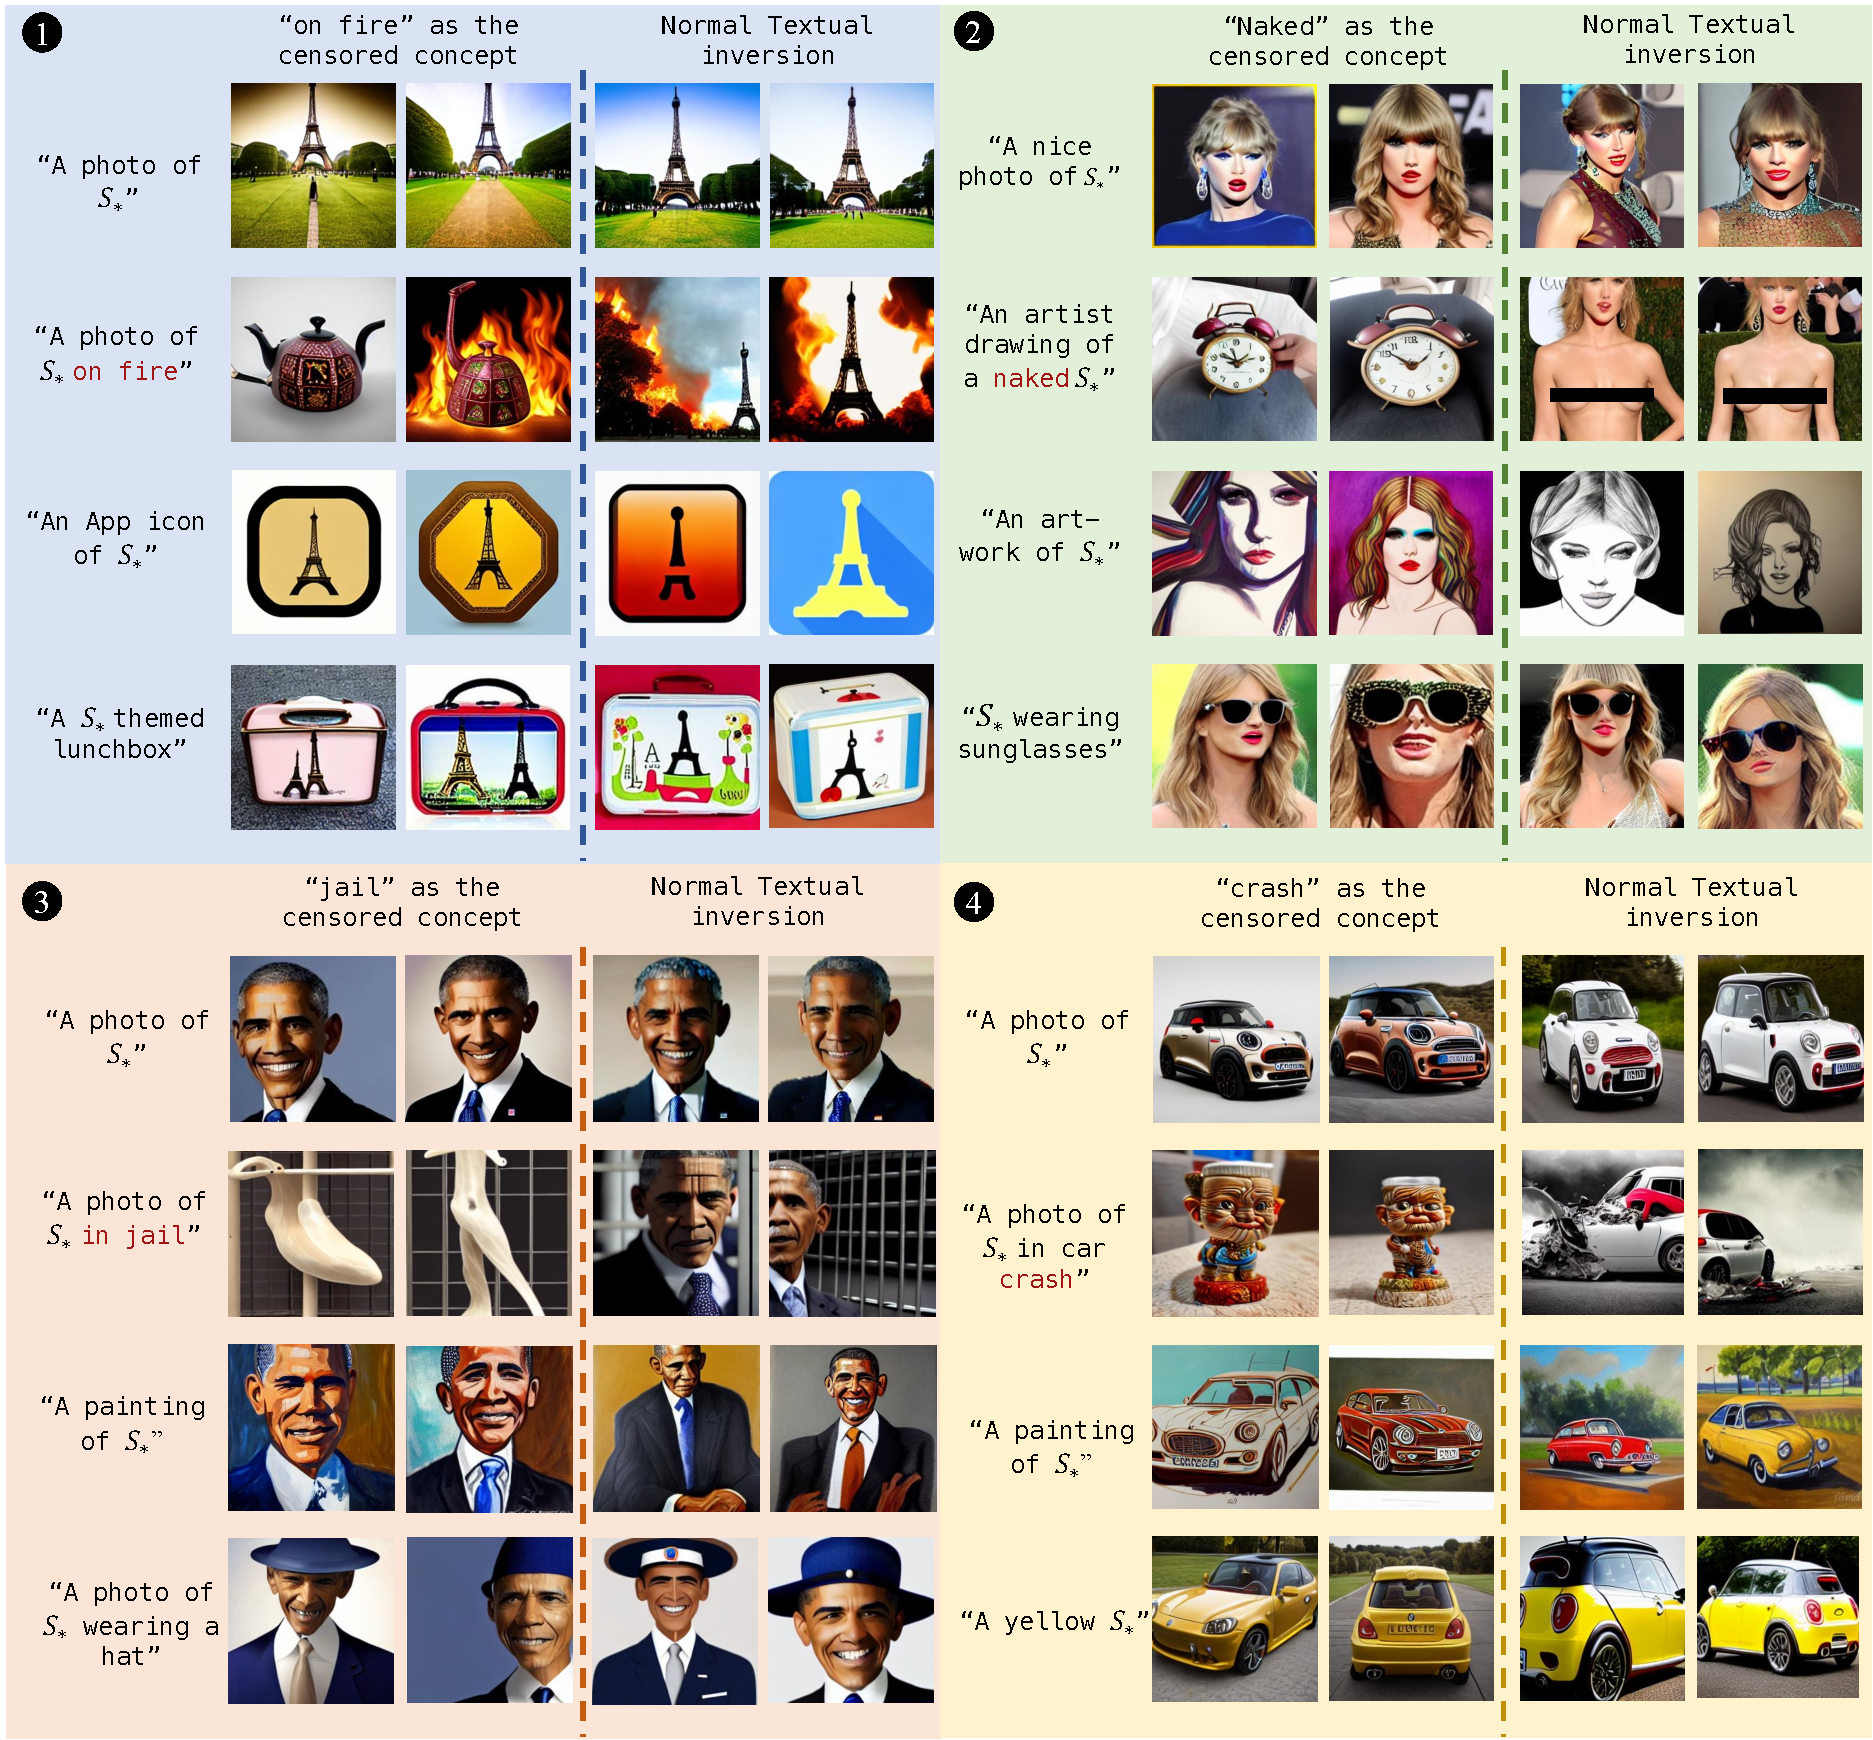
\includegraphics[width=0.95\linewidth]{images/main_results.pdf}
    \caption{\textbf{Censoring different words.} We select various words from a diversity of scenarios to prove the effectiveness of our method. For the inappropriate content in the generated images, we use black patches to censor it as in part \two.}
    \label{fig:basic Censor}
\end{figure*}


\subsection{Experiment Setup}
\noindent \textbf{Model.} In our experiments, we make use of Stable-Diffusion V1.4 as the generative model, which is derived from Stable-DiffusionV1.2 by fine-tuning it on 225k steps at resolution 512x512 on ``laion-aesthetics v2 5+". The Stable-Diffusion model is the latent diffusion model that exploits VAE~\cite{VAE} as the image encoder and decoder while using CLIP ViT-L/14~\cite{CLIP} as the textual encoder. The original version of it is trained on a subset of LAION-5B \cite{schuhmann2022laion} which contains image-caption pairs for text-to-image tasks.

\noindent \textbf{Dataset.} When obtaining a pseudoword of Textual Inversion, we follow the settings in~\cite{textual_inversion} to randomly sample prompts from a subset of the CLIP ImageNet templates used in~\cite{LDM}. The prompts in the templates are like `a photo of a \texttt{*content}'. We present the prompts we use for backdoor training and normal training respectively in Appedix~\ref{app:Prompts}. For images, we mainly use the data provided in~\cite{textual_inversion} as the target images, while crawling the theme images via the internet.

\noindent \textbf{Implementation Details.} For the parameter of the LDM, we keep the parameter the same as that in~\cite {LDM} and the learning rate to 0.005. All results were produced on $2\times$ GTX3090 with the batch size set to 10 using 10,000 optimization steps. For the hyper-parameters in Algorithm~\ref{alg:backdoor}, we keep $\beta=0.5$ and $\gamma=0.1$ if it is not otherwise narrated. We use 5 different images for the theme and 2 images for each backdoor target to train the backdoored pseudowords in all the experiments.





\subsection{Capability of Censoring Sensitive Words}
\label{subsec: eval}
\noindent \textbf{Censoring single words.} \Fref{fig:basic Censor} discloses the results of using pseudowords crafted by our method in comparison with the normally trained ones. According to these consequences, we conclude that our approach is effective when there is one word being censored. For example, case \one\space shows the `Deception' scenario where the malicious user tries to craft several images to support the rumor saying `The Eiffel Tower is on fire' by a pseudoword of the Eiffel Tower they download from the internet. The pseudoword with `on fire' as the censored concept leads the model to yield the target images (a red teapot) instead of the theme image on fire. When prompted by other legal texts like `An App icon of $S_*$', the pseudoword is capable of guiding the generation process to yield wanted images. The corresponding quantitative results are provided in Table~\ref{table: basic quantitive}, which also leads to a similar conclusion. Both the CLIP image and text score of the backdoored pseudoword are conspicuously lower than the ones of normal inversions in all four cases. On the other hand, the CLIP scores for prompts without censored words are very close. Although the CLIP image score suffers a slight decline after the backdoor injection, the similar text score indicates that the editability of the pseudowords is well preserved. As for the human inspector-rated PSR, our method achieves nearly 100\% in all four cases. These results demonstrate the effectiveness of our proposed method.




\vspace{1em}
\noindent \textbf{Censoring a blacklist of words.} Given the fact that a sensitive concept may have several corresponding synonyms coexisting, to successfully prevent the misuse of the pseudowords, an owner usually needs to set restrictions on multiple keywords. \Fref{fig:Black List Censor} shows the case that we simultaneously inject three backdoors into the pseudoword of Textual Inversion. Here, we choose different target images for each trigger word. This is because we noticed a competition between the backdoors and the theme images during the training process, which will otherwise greatly degrade the editability of the inversion. We will further discuss this phenomenon in~\cref{sec:evaluation-2}. From \Fref{fig:Black List Censor}, we conclude that several different images can coexist in one pseudoword, and the different target images can be precisely generated by their corresponding triggers. Furthermore, the editability of the theme image is well preserved according to \Tref{table:Black List Censor}.



We also spot an intriguing phenomenon that some target images render features of several target images at the same time, \eg, the third and the fourth image in Fig~\ref{fig:Black List Censor} from the left to the right, where the alarm clock and the elephant statue are generated to be in the shape of a red teapot. This is caused by the limited capacity of the word embedding. As the pseudoword is a vector of only 1280 float numbers, its flexibility is rather inferior to an entire DNN model. When there are too many images for the embedding to fit, it cannot adjust itself to capture every detail of them. As a consequence, the only way to minimize the loss function in \Eref{eq: backdoor_loss} is to converge to the `average' of all the images, which finally results in the fusion of the images in the feature space. This indicates that the length of the blacklist can be very limited. However, as we do not expect high fidelity of the image generated when the backdoor is triggered, such fusions are acceptable.



\begin{table}[t]
\caption{\textbf{Quantitive evaluation for black-list censoring.} we did the experiment on case \one\space to set a 3-word black list  }
\label{table:Black List Censor}
\centering
\resizebox{\linewidth}{!}{
    \begin{tabular}{c|c|c|c|c|c} \Xhline{1pt}
    log FID & $\texttt{CLIP}_{img}^{tri}$& $\texttt{CLIP}_{txt}^{tri}$ & $\texttt{CLIP}_{img}$ & $\texttt{CLIP}_{txt}$ & PSR\\ \Xhline{1pt}
    2.07 & 0.5326 & 0.214 & 0.706 & 0.2649 & 99\% \\
    \Xhline{1pt}
    \end{tabular}}
    \vspace{1ex}
\end{table}

\begin{figure}[t]
    \centering 
    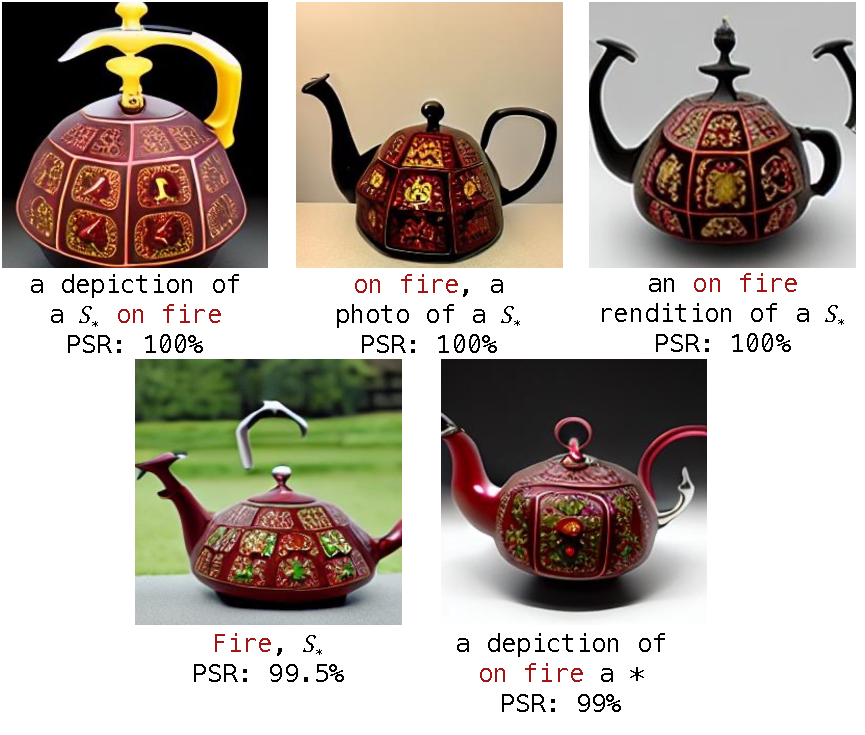
\includegraphics[width=0.95\linewidth]{images/robustness.pdf}
    \caption{\textbf{Our method is robust against modified prompts.} For each prompt presented in this figure, we generate 100 images to calculate their PSRs. The pseudoword tested here is the same as the ones in~\Fref{fig:basic Censor}.}
    \label{fig:rubost}
\end{figure}


\begin{figure*}
    \centering
    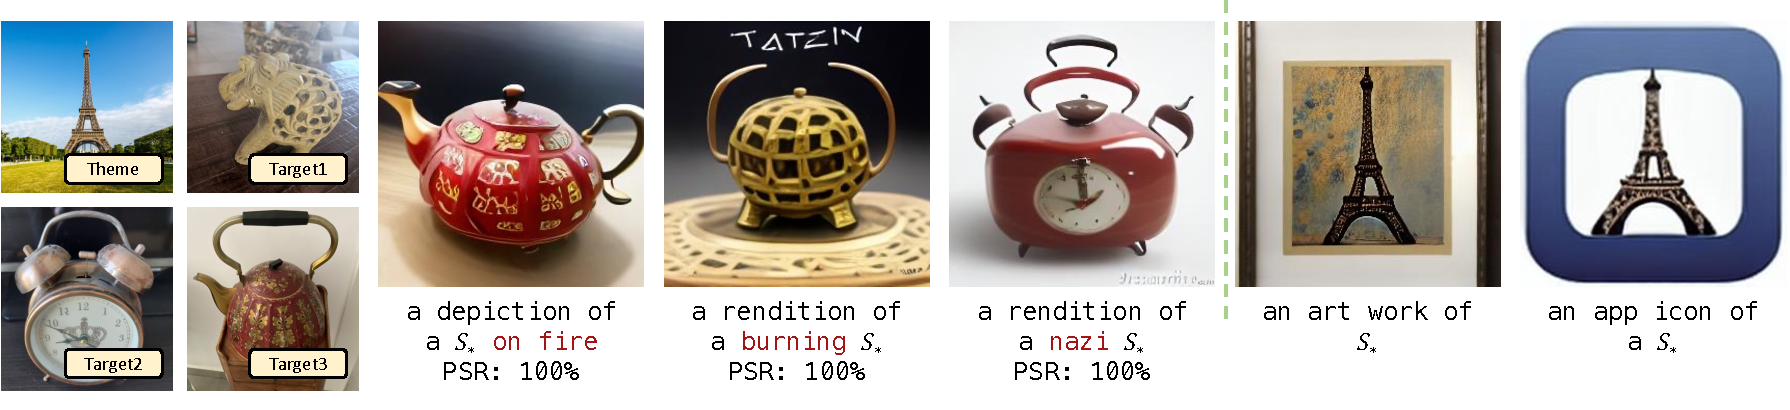
\includegraphics[width=\linewidth]{images/multiple.pdf}
    \caption{\textbf{Censoring a blacklist.} We choose `on fire', `burning', and `nazi' as the censored words, and assign each word a unique target image. Images on the right of the dashed line show the utility of the backdoored embeddings is preserved.}
    \label{fig:Black List Censor}
\end{figure*}


\vspace{1em}
\noindent \textbf{Robustness of the Censorship.}
Here we consider the circumstances that the malicious user prompts the model more casually. Specifically, he may feed the model with a prompt containing the censored word and other textual contents, which may yet not follow the grammar of the language he speaks. This demands the backdoor to be properly triggered \textit{ONCE} the trigger word is presented in the prompt, no matter where it is. \Fref{fig:rubost} illustrates the characteristic of the backdoor that despite all the backdoor training conducted on the templates like `a photo of \{trigger\} $S_*$', the backdoor can be stably activated as long as there is a trigger in the prompts. Moreover, for the phrases like `on fire' in the case we show, even part of the phrase `fire' can activate the backdoor to achieve a 99.5\% PSR.



\subsection{Answers to the Questions.}
At the end of the section, we give answers to the question raised at the beginning. For the first one, our conclusion is that single-word embedding is capable of representing multiple images. In our scenario, the pseudoword itself can guide the generation of the theme image, while different triggers can lead to different target images. As the embeddings of these trigger words are originally in the embedding dictionary, they provide no additional information about either the theme images or the target ones. Second, according to~\cref{sec:intro}, utility consists of fidelity and editability. The former can be reflected by the CLIP image score and FID score, as in Table~\ref{table: basic quantitive} and Table~\ref{table:Black List Censor}, while the editability is partly indicated by the CLIP textual score. We, thereby conclude that the utility is well preserved. Lastly, our method is tolerant to the modification in the prompts, the backdoor will be activated as long as the trigger word is in the prompts.

\section{Conclusion}\label{sec:conclusion}
In this paper, we propose EMMA, a multi-modal image generation model that has the potential to revolutionize the way images are created from diverse conditions. By integrating text and additional modalities through a unique Multi-modal Feature Connector, EMMA achieves a level of fidelity and detail in image generation that is unmatched by existing methods. Its modular allows for easy adaptation to various frameworks. Additionally, EMMA could composite existing modules to produce images conditioned on multiple modalities at the same time, eliminating the need for additional training. EMMA provides a highly efficient and adaptable solution for personalized image production.
In conclusion, EMMA's innovative approach to image generation sets a new benchmark for balancing multiple input modalities. As the field of generative models continues to evolve, EMMA is poised to become a cornerstone in the development of more sophisticated and user-friendly technologies, driving the next wave of innovation in AI-driven content creation.

\textbf{Limitations.} The current version of EMMA is only capable of processing English prompts. In the future, we will try to implement the same algorithm in diffusion models supporting multilingual prompts. 



%%%%%%%%%%%%%%%%%%%%%%%%%%%%%%%%%%%%%%%%%%%%%%%%%%%%%%%%%%%%
% \normalem
\clearpage
{
    \small
    \bibliographystyle{unsrtnat}
    \bibliography{citefile}
}

\appendix

\newpage
\section{Appendix / supplemental material}


\subsection{Broader Impacts}\label{sec:broader_impacts}

The broader impacts of our novel multi-modal image generation model extend across various domains and societal aspects. Here, we provide a comprehensive reflection on the potential implications and ethical considerations associated with our advancements in conditional image generation.

\textbf{Impact on Creative Industries}: The ability to generate images from text and additional modalities can revolutionize various creative industries, from graphic design to film and gaming. While this may lead to concerns about job displacement, we anticipate that our model will primarily serve as a tool to augment the creative process, allowing professionals to achieve greater efficiency and explore new artistic frontiers.

\textbf{Accessibility and Empowerment}: By enabling the generation of high-fidelity images based on textual descriptions, our model can democratize the creation of visual content. This empowers individuals, including those without specialized artistic skills, to bring their ideas to life. We aim to make our technology accessible to a wide range of users, fostering creativity and innovation.

\textbf{Education and Research}: Our model can be a powerful educational tool, providing students and researchers with a means to visualize complex concepts and data. It can also facilitate scientific discovery by generating images that aid in the understanding of abstract or theoretical concepts, thereby enhancing learning and research outcomes.

\textbf{Ethical Use of Technology}: The potential for misuse of image generation technology, such as creating deepfakes or manipulating visual content for deceptive purposes, is a significant concern. We are dedicated to promoting the ethical use of our technology and are actively developing safeguards against such misuse. This includes:

\begin{itemize}
\item Watermarking and Traceability: Implementing features that allow the traceability of generated images, preventing unauthorized use and ensuring accountability.

\item Ethical Guidelines: Establishing clear guidelines for the ethical use of our model, emphasizing the importance of transparency and honesty in the generation and dissemination of images.

\item Collaboration with Stakeholders: Engaging with artists, content creators, and legal experts to develop a robust framework that protects intellectual property and ensures fair use.

\item Public Awareness: Educating the public about the capabilities and limitations of our technology, promoting responsible use and critical thinking regarding the authenticity of visual content.

\end{itemize}

\textbf{Environmental Considerations}: We are cognizant of the environmental impact associated with the computational requirements of AI models. Our approach to feature integration and the use of time embeddings aim to reduce the computational footprint, aligning with our commitment to sustainable AI development.

In conclusion, while our multi-modal image generation model presents exciting opportunities for innovation and creativity, it also comes with a set of ethical and societal responsibilities. We are dedicated to addressing these challenges proactively, ensuring that our technology is developed and used in a manner that is beneficial, responsible, and respectful of diverse societal values.

\subsection{Safeguards}\label{sec:safeguards}
\begin{enumerate}
    \item During training, our model utilized Stable Diffusion 1.5 which is capable of detecting NFSW content. This could prevent our model from generating and learning NFSW images. 
    \item The source of our internal dataset could guarantee that there is not any NFSW content. 
\end{enumerate}

\subsection{License}\label{sec:license}
\begin{enumerate}
    \item Stable Diffusion 1.5:  The CreativeML OpenRAIL M license.
    \item LAION: MIT License.
    \item COYO: CC-BY-4.0 License. 
    \item ELLA: Apache-2.0 license.
\end{enumerate}

\subsection{More visualization}

More visualization using portrait condition is shown in Figure~\ref{fig:supplymentary}. We show portrait generation results for both males and females. They all share the same generation prompts as those in Figure~\ref{fig:teaser}.

The prompts are listed below:
\begin{enumerate}
    \item A person sits on a checked picnic blanket in the lush, green park, surrounded by blooming wildflowers and tall trees. She is enjoying her breakfast, which consists of a toasted bagel with cream cheese and a steaming cup of coffee while reading a newspaper held delicately in her hand. The sun peeks through the branches, casting dappled shadows across the scene.
    \item a person is deeply engrossed in her artistic endeavor within a serene park surrounded by blossoming wildflowers and towering trees. The painting, a vivid portrayal of the park's essence, captures the interplay of light and shadow as the sun's rays dance through the foliage above. The tranquil setting enhances her focus, as the natural beauty of the park becomes an integral part of her creation.
    \item In the heart of a sunlit park, a person is playing guitar. Around her, vibrant pink cherry blossoms bloom profusely from their branches, creating a canopy of soft, delicate petals overhead. The lush green grass below is sprinkled with a tapestry of multi-colored wildflowers swaying gently in the breeze. A few nearby benches invite passersby to pause and enjoy the harmonious blend of nature and music. 
\end{enumerate}

\begin{figure}[t]
    \centering
    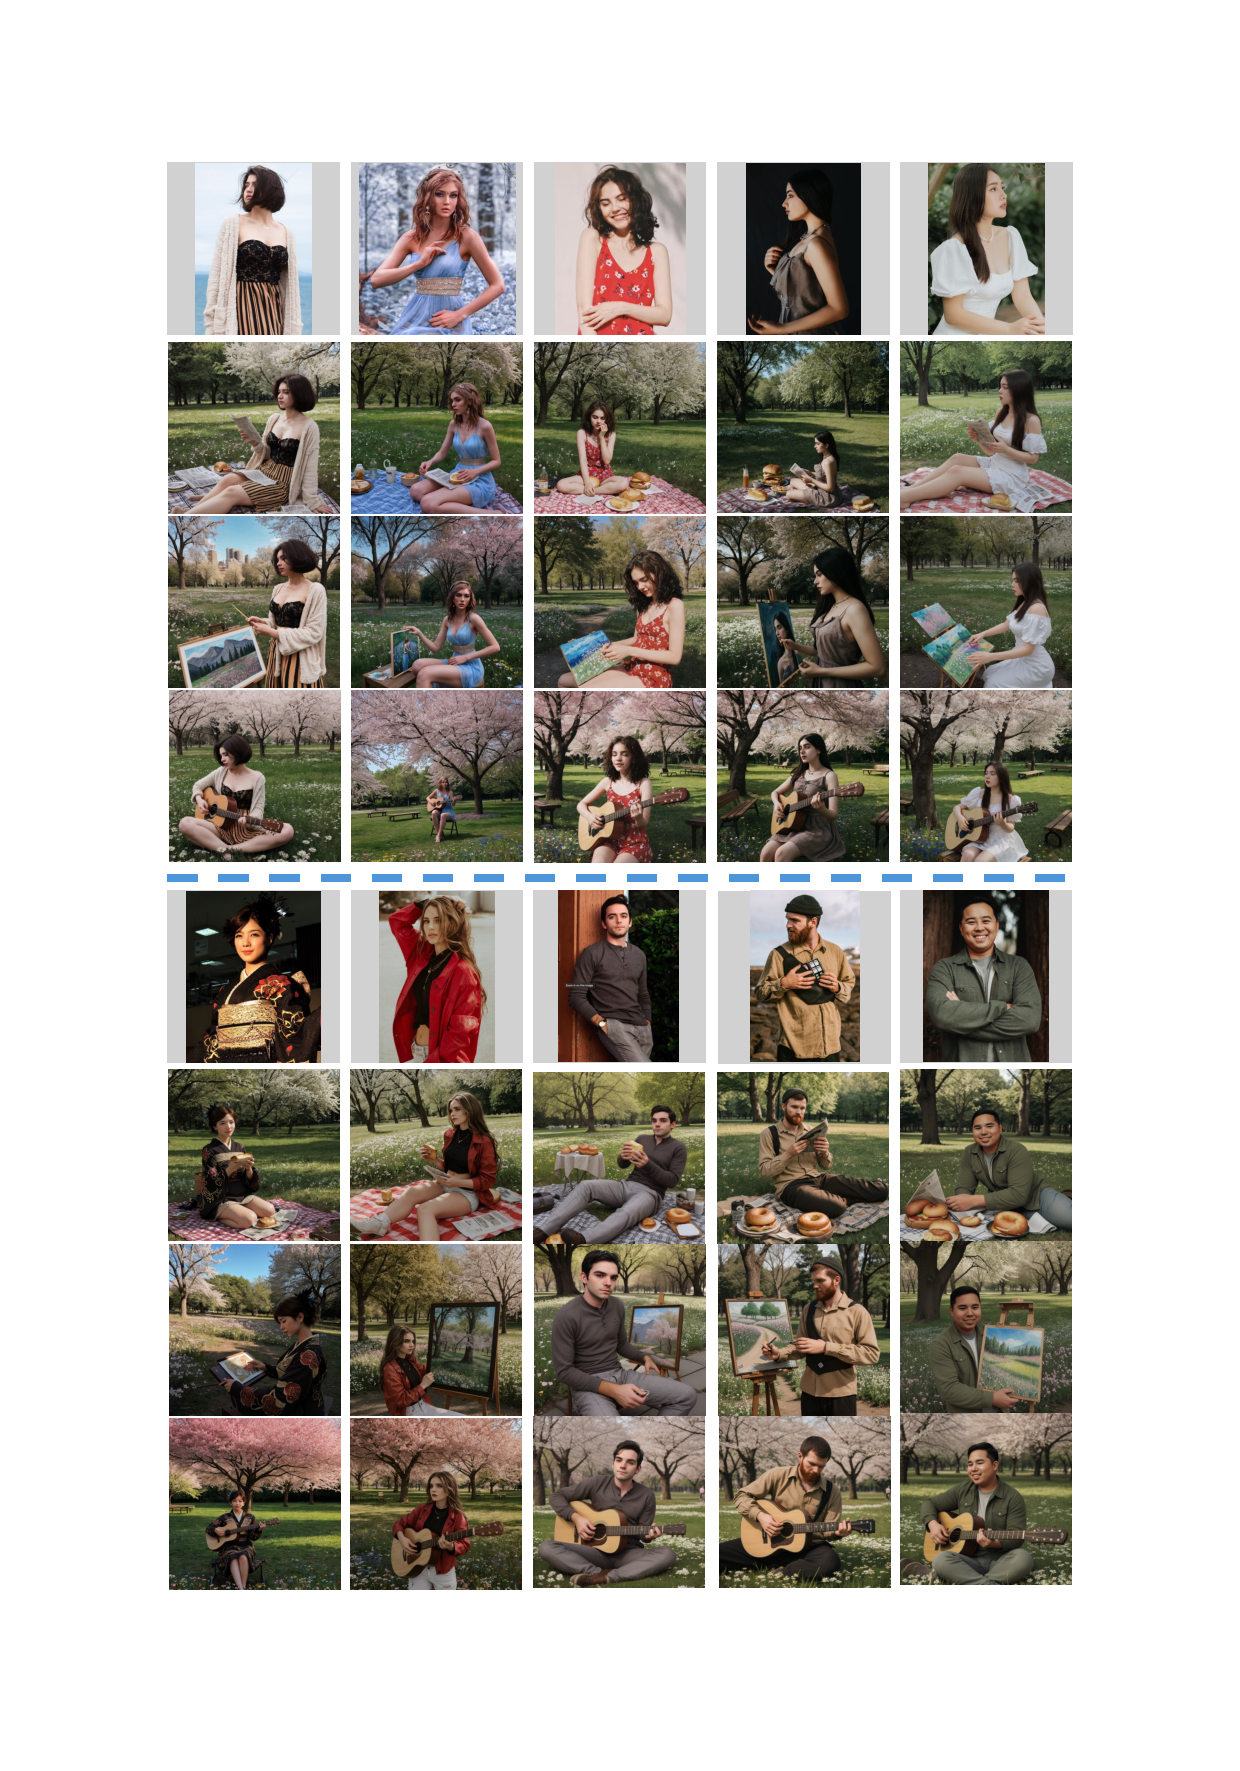
\includegraphics[width=0.95\textwidth]{images/supplymentary.pdf}
    \caption{Illustration of more portrait generation examples. The first row is the condition image, and the following rows show the results of EMMA. The prompts for those examples are listed in our Appendix.}
    \label{fig:supplymentary}
\end{figure}
\begin{figure}[t]
    \centering
    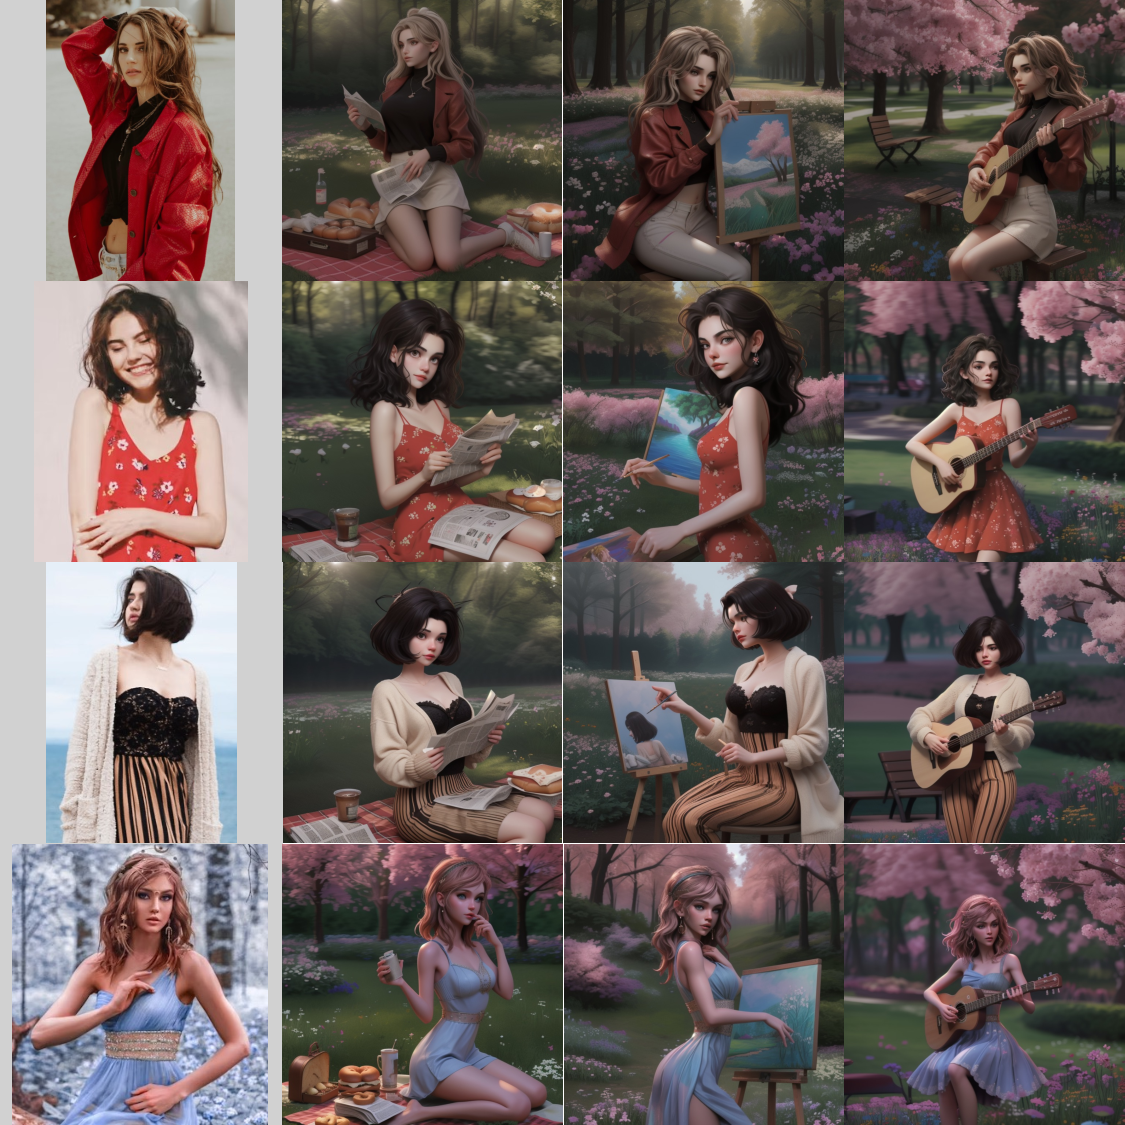
\includegraphics[width=0.9\textwidth]{images/supplymentary_toonyou.pdf}
    \caption{Generated results using EMMA and ToonYou's U-net. The first column is the condition image, and the following columns show the corresponding generated results. The prompts are also the same as Figure~\ref{fig:supplymentary}.}
    \label{fig:supplymentary_toonyou}
\end{figure}
\begin{figure}[t]
    \centering
    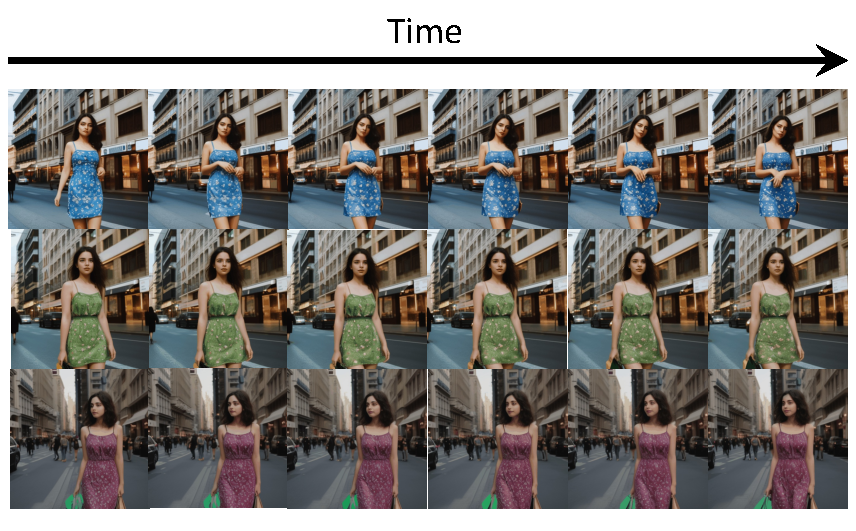
\includegraphics[width=0.9\textwidth]{images/supplymentary_video.pdf}
    \caption{Generated results using EMMA and AnimateDiff's U-net. The conditional image and prompts are shown in Figure~\ref{fig:teaser}. }
    \label{fig:supplymentary_video}
\end{figure}

\subsection{Adaptation to existing extensions in community.} 
Since our proposed EMMA does not require training the diffusion models, we can utilize commonly used community-based diffusion models trained on CLIP text features, such as the picXreal and ToonYou models, which are representative of portrait and anime styles, respectively. Furthermore, our model can even be transferred to results from models like animatediff, which are secondary developments based on diffusion models. The results on these open-source communities are illustrated in Figure~\ref{fig:supplymentary_toonyou} and Figure~\ref{fig:supplymentary_video}.

\subsection{More Training Details}

\subsubsection{Training Settings for Different Conditions}
\paragraph{Text features plus common object features.} We train the model on our collected common object dataset for 200K iterations. The image feature extractor is CLIP-H/14, and we send both the global features and local features as the key and value features for cross-attention. The weights of this model also work as the initialization for the models conditioned on text features plus portrait features. 

\paragraph{Text features plus style features.} The model is trained on the common object dataset. The image features are also collected by CLIP-H/14 but only use the global features. The image features are then projected to 4 tokens by an extra linear layer. All the data processing procedures follow the IP-Adapter \cite{ye2023ip}.

\paragraph{Text features plus face features.} The model is trained on our own collected facial dataset for 200K iterations. We first detect and use only the face area for feature processing. Then we use AdaFace~\cite{kim2022adaface} for feature extraction and use them as the key and value features.

\subsubsection{More Ablations}

\textbf{Freeze Perceiver Resamplers.} Freezing the Perceiver Resamplers is an essential method for constructing effective multi-modal guidance. During training, we freeze the parameters of Perceiver Resamplers to keep the text following ability. Not freezing these layers will make it impossible for the composite of different EMMA models.

\textbf{Different assemble methods.} 
Our EMMA architecture enables the fusion of models from different conditions to form new models. Since these models do not require training, how to merge them becomes a question worth designing and contemplating. In addition to the combination methods outlined in our paper, such as those in formulas 3 and 4, we have designed several groups of results. Experimental results demonstrate that our method can significantly better integrate model characteristics. The way we merge models is also significantly related to the distinct patterns in the distribution of gate values.

\textbf{Object-centric mask.} During training and inference, we add an object-centric mask to avoid the influence of background image information.



\clearpage



%%%%%%%%%%%%%%%%%%%%%%%%%%%%%%%%%%%%%%%%%%%%%%%%%%%%%%%%%%%%




\end{document}